\documentclass{article}

% always load these packages
\usepackage{amsmath,amsfonts,amssymb,amsthm}
\usepackage{mathtools}
\usepackage{graphicx,float}
\usepackage{todonotes}
\usepackage{hyperref}
\usepackage{dirtytalk}
\hypersetup{
    colorlinks,
    citecolor=black,
    filecolor=black,
    linkcolor=black,
    urlcolor=black
}
\usepackage{nth}
\usepackage[framed,numbered,autolinebreaks,useliterate]{mcode}


% reciprocal hyperbolic trigonometric functions
\DeclareMathOperator\csch{csch}
\DeclareMathOperator\sech{sech}

% sign function
\DeclareMathOperator\sign{sign}

% more readable real part and imaginary part functions
\renewcommand\Re{\mathrm{Re}}
\renewcommand\Im{\mathrm{Im}}

% matrix environment for vectors or matrices where elements are centered
\newenvironment{mat}{\left(\begin{array}{ccccccccccccccc}}{\end{array}\right)}
\newcommand\bcm{\begin{mat}}
\newcommand\ecm{\end{mat}}

% common sets of numbers
\newcommand\reals{\mathbb{R}}
\newcommand\complex{\mathbb{C}}
\newcommand\ints{\mathbb{Z}}
\newcommand\nats{\mathbb{N}}

% other common symbols
\newcommand\matlab{{\sc matlab}}
\newcommand{\goto}{\rightarrow}
\newcommand{\bigo}{{\mathcal O}}


\usepackage{fullpage}

\usepackage[titletoc,title]{appendix}

%\renewcommand{\lstlistingname}{Code}

\title{AMATH 582: Final Project}
\date{March \nth{16}, 2017}
\author{Lee Burke \\ Taylor Cunnington}

\renewcommand{\thesection}{Sec.~\Roman{section}}
%\renewcommand{\thesubsection}{\arabic{section} (\alph{subsection})}
%\renewcommand{\thesubsubsection}{\arabic{section} (\alph{subsection}) (\roman{subsubsection})}

\usepackage{chngcntr}
\counterwithout{figure}{section}

\begin{document}
\maketitle
\abstract{
}
\section{Introduction and Overview}
Classifying bank transactions as fraudulent is a difficult task: (1) data is highly sensitive and so difficult to come by, (2) relevant features are not always clear, and (3) classification algorithms have trouble with unbalanced data where fraud is much less common than honest purchases. 


To answer the first problem, we analyze real credit card data from a challenge on \href{kaggle.com}{link?}. However, to preserve confidentiality, the features have been obscured by a singular value decomposition (SVD): we are given $U\Sigma$ if the original data $A=U\Sigma V^\ast$ in the usual SVD. That is, we have no say in the second problem, feature extraction. Indeed, the PCA modes have no discernable structure, and decay slowly. Instead, we focus on classifying skewed data.

That popular algorithms have trouble with skew is, in some sense, expected: minimizing the error rate inherently favors the major class. Guessing the larger class every time is already above $50\%$ accuracy. In addition, overall error is not the metric we care most about: false positives (mistakenly flagging a transaction as fraud) have much lower cost to the bank and consumer than false negatives (someone gets away with fraud). Our dataset is a great example of imbalanced data. Only $0.17\%$ of the data points are classified positive. It is difficult to improve on $99.83\%$ accuracy!

We apply several methods learned in lecture, including linear discriminant analysis (LDA), a binary classification tree (BCT), and a support vector machine (SVM). A new method is used to reduce the skew in the class sizes in combination with LDA. We focus especially on how to compare the performance of these classifiers, because common performance metrics may not be as descriptive with high-cost, highly-skewed data.

\section{Theoretical Background}
A brief theoretical exploration of classification and its evaluation is given below.

\subsection{Classification}
\subsubsection{Linear Discriminant Analysis}
The LDA algorithm builds normal probability distributions for each class with mean and covariance parameters $\left({\vec {\mu }}_{0}, \sigma_{0} \right) \left({\vec {\mu }}_{0}, \sigma_{0}\right) and \left({\vec {\mu }}_{1},\sigma_{1}\right) \left({\vec {\mu }}_{1}, \sigma_{1}\right)$
These are referred to as the prior distributions. Classifying subsequent observations is then potentailly just a matter of comparing their probability of being in class 0 or 1 and applying a threshold.
MATLAB actually attempts to minimize the cost function:
\begin{equation}
\hat{y}=\arg\min_{y=1,...,K}\sum_{k=1}^{K}\hat{P}(k|x)C(y|k)
\end{equation}
where $\hat{y}$ is the predicted probability. $K$ is the number of classes. $\hat{P}$ is the posterior probability of class $k$ for a given observation $x$, and $C(y|k)$ is the cost of misclassifying $k$ as $y$.
$\hat{P}$ is determined from Bayes rule:
\begin{equation}
\hat{P}(k|x)=\frac{P(x|k)P(k)}{P(x)}
\end{equation}
Here the posterior probability that $x$ is in class $k$ is what LDA estmiates from the training data.
$P(k)$ and $P(x)$ are readily calcuated the from the data.
Note that for the case of an extremely small minority class such as ours $P(n)$ will be extremely small (where $k=n$); this means that $\hat{P}(n|x)$ will be small as well.
This is a source of bias for LDA toward the majority class.

\subsubsection{Binary Classification Trees}

\subsubsection{Support Vector Machines}

\subsection{Handling Class Skew}
There are some known methods for improving performance when classifying imbalanced data. The four common solution types are given here:
\begin{enumerate}
\item Under-sampling -- Removing data from the larger class to balance the class sizes.
May lead to a poorer choice of decision line due to losing data at the border of the classes.
\item Oversampling -- Adding extra observations on top of existing minority class observations to balance out the class sizes.
May lead to overfitting with some classification models.
\item Synthetic data generation -- Generating artificial data from your existing data to balance classes.
Generated data generally stays within the n-dimensional volume that minimally encloses the existing data.
\item Cost functions-- Classification algorithms use cost functions (decision functions) to define their decision boundaries.
With imbalanced data you would set the misclassification of the minority class to be much more costly, to encourage the algorithm to classify them correctly more often than the majority class.
\end{enumerate}
The first three attempt to reduce the imbalance by reducing the number of majority data point or increasing the number of minorty data points.
These methods deal with the data only, not the classifier.
The final option does alter the classifier however, to try to make it classify the minority class more reliably.

\subsection{Performance Evaluation}

\subsubsection{Receiver Operating Characteristics (ROC) Curve}

\subsubsection{Precision/Recall (PR) Curve}
%
%It's not just accuracy that serves as a poor metric in this task.
%Precision and Recall are two common measures.
%Plotting the former on the y-axis and the latter on the x-axis gives you Precision-Recall (PR) curves, which are often used to evaluate algorithms.
%Recall is the fraction of positive entries that you correctly identified as positive: tp/(tp+fn).
%Precision is the fraction of entries that were actually positive out of all the ones you guessed were positive: tp/(tp+fp).
%
%In our case we want to optimize for recall over precision.
%That is, when we are given an input that is actually positive we want to correctly predict as much as possible that it is positive, even if that means we end up with false positives.
%If we get false positives that lowers our precision, but since false negatives are more costly than false positives here we can accept potentially many more false positives.
%
%
%For the reason above precision is not a good metric for this task.
%For the functionality we want to optimize we will likely see precision increase over a simple majority class classifier, but we can't really be sure of the exact relationship.
%A better metric would be one that is guaranteed to decrease monotonically as we approach our ideal of perfect recall, regardless of what happens to precision.
%
%A metric that does work well is the Area Under the Precision-Recall Curve (AUPRC)...

\section{Algorithm Implementation and Development}

As stated above our data was prepared and features provided as U columns of the SVD decomposition, so we did not alter or clean the data.
We created a \say{full} data matrix $X$ from the 28 columns of U and the amount of the transaction.
We used standard Z-score of the $X$ matrix, $Z$, for all implementations of the LDA classifier.

Then we split the data for cross validation... or did we do k-fold validation??

Using LDA as our classification algorithm we compared the synthetic data generation and alternate cost function approaches to the default algorithm.
For synthetic data generation we chose to use ADASYN (Adaptive Synthetic Sampling Approach for Imbalanced Learning) a generation algorithm similar to the well known SMOTE (Synthetic Minority Over-Sampling Technique) algorithm, which is ADASYN's precursor.
The goal of both is to improve the class balance by increasing the number of minority class members.
SMOTE places synthetic data between existing data points randomly (linear interpolation), with no preference shown to any specific points.
ADASYN does the same thing but places more synthetic data points close to the boundary between classes because those are the original data points that are more difficult to learn.
(Does this favor decision trees or SVMs or something? I imagine that all this would do for an LDA is to move the mean of the minority gaussian close to the boundary...
SMOTE might be better here...)

We also tried changing the cost function of our LDA model to discourage FNs.
Since LDA works by creating probability distributions the cost comes into play only when making predictions.
Each observation that it is trying to predict has a calculated posterior probability.
It tries to minimize the "classification cost"--this is a decision cost function.
Unfortunately if an observation has an extremely small posterior probability then even with a vary large cost for miscalculating that observation it may not change the classification cost by much, meaning there will be little change to the resulting prediction.

\section{Computational Results}

GIVE BASELINE LDA RESULTS

Altering the prediction cost function does not make a difference in our case.
Weighting false negatives as very costly makes very little difference, even when the cost of a false negative is $10^8$ as costly as a false positive.
This seems odd, since we only expect class $p$ to be about 500 times as likely class $n$ ($P(p) \approx 500 \times P(n)$).
There must be something else going on...
PERFORMANCE MATRICS

Synthetic data generation did improve recall. As expected this came at the cost of precision and accuracy.
PERFORMANCE METRICS

\begin{figure}[!htb]
	\centering
	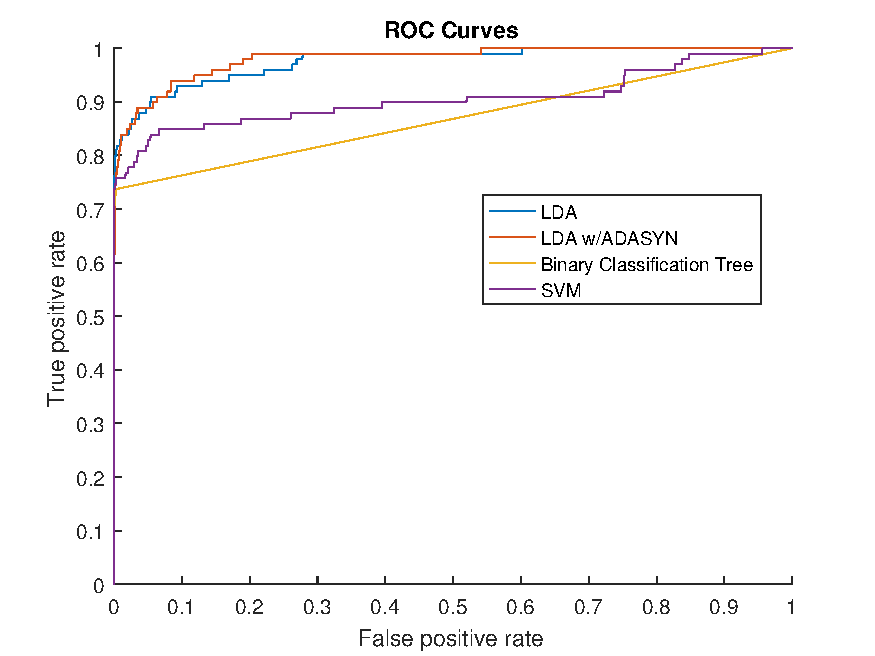
\includegraphics[width=0.8\textwidth]{ROC}
	\caption{}
	\label{fig:roc}
\end{figure}
\begin{figure}[!htb]
	\centering
	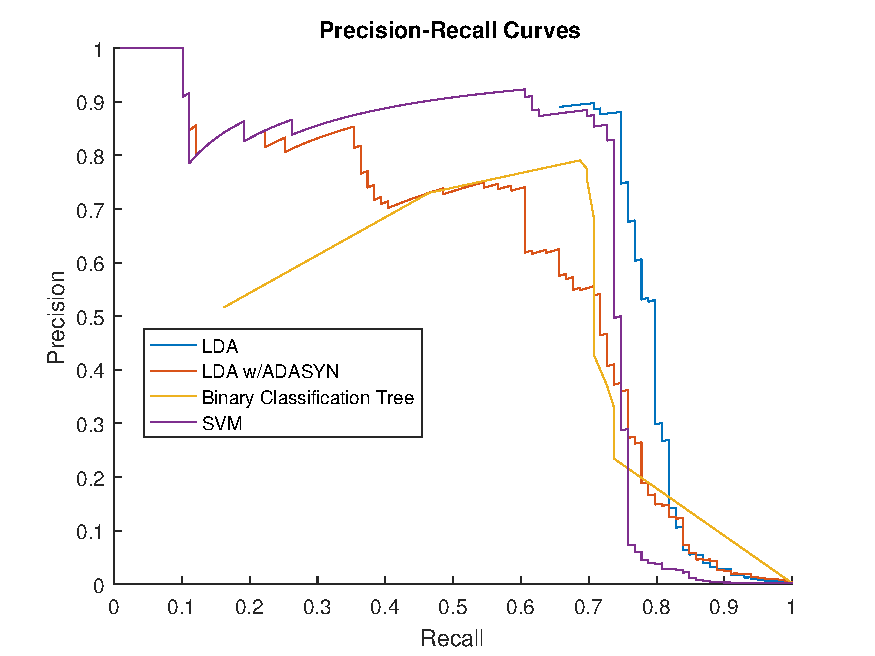
\includegraphics[width=0.8\textwidth]{PR}
	\caption{}
	\label{fig:pr}
\end{figure}

\begin{table}[!htb]
	\centering
	\caption{}
	\label{tab:area}
	\begin{tabular}{r|c|c}
		& AUCs & AUCPR \\
		\hline
		LDA & 0.976 & 0.124 \\
		LDA w/ADASYN & 0.980 & 0.538 \\
		Binary Classification Tree  & 0.868 & 0.416 \\
		SVM & 0.905 & 0.660
	\end{tabular}
\end{table}

\section{Summary and Conclusions}

\clearpage
\begin{thebibliography}{9}
  
\bibitem{dalpozzolo}
\texttt{https://www3.nd.edu/~dial/publications/dalpozzolo2015calibrating.pdf}

\bibitem{AUC}
wiki: ROC, AUC

\bibitem{machinelinearningmastery}
\texttt{http://machinelearningmastery.com/classification-and-regression-trees-for-machine-learning/}

\end{thebibliography}

\begin{appendices}
\section{MATLAB functions used and brief implementation explanation}
\begin{itemize}
	\item \texttt{fitctree}
	\item \texttt{fitcsvm}
	\item \texttt{fitcdiscr}
	\item \texttt{ADASYN}
	\item \texttt{predict}
	\item \texttt{perfcurve}
\end{itemize}

\section{MATLAB codes}
\lstinputlisting[caption=Main, label=code:main]{../main.m}
\lstinputlisting[caption=Split data into training and test sets, label=code:splitBinaryClassData]{../splitBinaryClassData.m}
\lstinputlisting[caption=Random permutation for indices, label=code:splitIndices]{../splitIndices.m}
\lstinputlisting[caption=Performance characteristics of a classification model, label=code:evaluate]{../evaluate.m}
\end{appendices}
\end{document}
